\documentclass[tikz, border=2pt]{standalone}

\usepackage{helvet}
\renewcommand{\familydefault}{\sfdefault}

\usepackage[EULERGREEK]{sansmath}
\sansmath
\usetikzlibrary{arrows.meta}

\begin{document}%

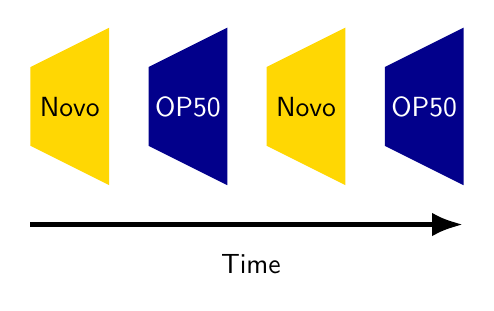
\begin{tikzpicture}[line width=2pt]
\tikzset{>={Latex[width=3mm,length=4mm]}}

% grid
% \draw[help lines] (-2, -5) grid (10, 15);

\definecolor{gold}{RGB}{255,215,3}

\definecolor{darkblue}{RGB}{2,0,139}

\draw [draw=none, line width=2pt, fill=gold] (0, 0) -- (1, 0.5) -- (1, -1.5) -- (0, -1) -- (0,0){};

\draw [draw=none, line width=2pt, fill=darkblue] (0+1.5, 0) -- (1+1.5, 0.5) -- (1+1.5, -1.5) -- (0+1.5, -1) -- (0+1.5,0){};

\draw [draw=none, line width=2pt, fill=gold] (0+3, 0) -- (1+3, 0.5) -- (1+3, -1.5) -- (0+3, -1) -- (0+3,0){};

\draw [draw=none, line width=2pt, fill=darkblue] (0+4.5, 0) -- (1+4.5, 0.5) -- (1+4.5, -1.5) -- (0+4.5, -1) -- (0+4.5,0){};

\draw [->, draw=black, line width=2pt, fill=gold] (0, -2) -- (5.5, -2);

\draw (2.8, -2.5) node{{\sf Time}};



\draw (0.5, -0.5) node[text=black]{{\sf Novo}};

\draw (2, -0.5) node[text=white]{{\sf OP50}};

\draw (3.5, -0.5) node[text=black]{{\sf Novo}};

\draw (5, -0.5) node[text=white]{{\sf OP50}};
\end{tikzpicture}


\end{document}